% //////////////////////////////////////// %
% /// Architecture web et relationnel //// %
\section{Architecture web et relationnel}
	%% Architecture classique
	\subsection{Architecture classique}
	\begin{frame}
		\frametitle{Architecture classique}

		\begin{figure}[htb]
			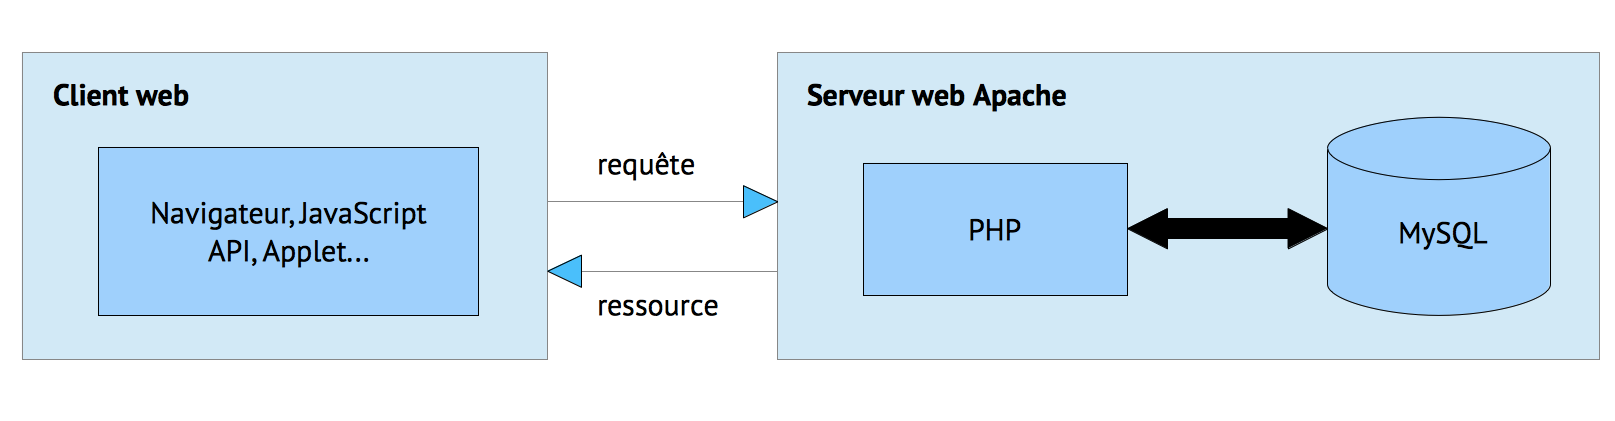
\includegraphics[width=1\textwidth]{images/LAMP.png}
		\end{figure}

		\begin{itemize}
			\item La plus commune : LAMP (Linux, Apache, MySQL, PHP) ;
			\item LEMP : Linux, Nginx, MySQL, PHP-FPM ;
			\item Stack JavaScript MEAN : MySQL (ou MongoDB), Express, AngularJS, Node.js.
		\end{itemize}

	\end{frame}

	%% Bilan architecture classique
	\subsection{Bilan architecture classique}
	\begin{frame}
		\frametitle{Bilan architecture classique}

		\textbf{Avantages :}
		\begin{itemize}
			\item Rapide à mettre en place (installation en un clic généralement) ;
			\item Optimisation possible, verticalement le plus souvent ;
		\end{itemize}

		\vspace{20px}

		\textbf{Inconvénients :}
		\begin{itemize}
			\item Il faut une expertise base de données.
		\end{itemize}

	\end{frame}

	%% Qu'est-ce qu'un ORM ?
	\subsection{Qu'est-ce qu'un ORM ?}
	\begin{frame}
		\frametitle{Qu'est-ce qu'un ORM ?}

		\begin{block}{Définition : ORM}
			L'\textbf{O}bject-\textbf{R}elationnal \textbf{M}apping est une technique qui simule une base de données orientée objet à partir d'une base de données relationnelle.
		\end{block}

		\vspace{5px}

		\begin{itemize}
			\item Fait la liaison entre le monde relationnel dans la couche stockage et le monde objet dans l'application ;
			\item Facilité de développement : pas besoin d'une connaissance poussée du SQL ;
			\item Facilite les interactions avec la base de données ;
		\end{itemize}

		\vspace{5px}

		\begin{alertblock}{Les limites des ORM}
			Toujours \textbf{beaucoup} moins performant que des requêtes SQL optimisées.
		\end{alertblock}

	\end{frame}